\documentclass[journal]{IEEEtran}
%
% *** GRAPHICS RELATED PACKAGES ***
%
\ifCLASSINFOpdf
  \usepackage[pdftex]{graphicx}
  % declare the path(s) where your graphic files are
  % \graphicspath{{../pdf/}{../jpeg/}}
  % and their extensions so you won't have to specify these with
  % every instance of \includegraphics
  % \DeclareGraphicsExtensions{.pdf,.jpeg,.png}
\else
  % or other class option (dvipsone, dvipdf, if not using dvips). graphicx
  % will default to the driver specified in the system graphics.cfg if no
  % driver is specified.
  \usepackage[dvips]{graphicx}
  % declare the path(s) where your graphic files are
  % \graphicspath{{../eps/}}
  % and their extensions so you won't have to specify these with
  % every instance of \includegraphics
  % \DeclareGraphicsExtensions{.eps}
\fi
\ifCLASSOPTIONcompsoc
  \usepackage[caption=false,font=normalsize,labelfont=sf,textfont=sf]{subfig}
\else
  \usepackage[caption=false,font=footnotesize]{subfig}
\fi
%
\usepackage{amsmath,amssymb}
\usepackage{color}
\newcommand{\red}[1]{\textcolor{red}{#1}}
\usepackage{ulem} % \sout{}
%
\begin{document}
%
% paper title
\title{Far-sidelobe Measurement of LiteBIRD \\ Low Frequency Telescope in 1/4-Scale}
%%%
%
% author names and IEEE memberships
% note positions of commas and nonbreaking spaces ( ~ ) LaTeX will not break
% a structure at a ~ so this keeps an author's name from being broken across
% two lines.
% use \thanks{} to gain access to the first footnote area
% a separate \thanks must be used for each paragraph as LaTeX2e's \thanks
% was not built to handle multiple paragraphs
%
\author{Hayato~Takakura, Yutaro~Sekimoto, Junji~Inatani, Shingo~Kashima, Hiroaki~Imada, Takashi~Hasebe, Toru~Kaga, Yoichi~Takeda, and~Norio~Okada%~\IEEEmembership{Life~Fellow,~IEEE}% <-this % stops a space
\thanks{H. Takakura is with Department of Astronomy, School of Science, University of Tokyo, Tokyo Japan e-mail: takakura@astro.isas.jaxa.jp}% <-this % stops a space
\thanks{H. Takakura, Y. Sekimoto, J. Inatani, T. Hasebe, T. Kaga, Y. Takeda and N. Okada are with Institute of Space and Astronautical Science (ISAS), Japan Aerospace Exploration Agency (JAXA).}% <-this % stops a space
\thanks{S. Kashima and N. Okada are with National Astronomical Observatory of Japan.}% <-this % stops a space
\thanks{H. Imada are with Laboratoire de l'Accélérateur Linéaire, Université Paris-Sud, CNRS/IN2P3, Université Paris-Saclay.}% <-this % stops a space
\thanks{Manuscript received XXXXX; revised XXXXX.}}
%%%
%
% The paper headers
\markboth{IEEE Transactions on Terahertz Science and Technology,~Vol.~XX, No.~X, November~2019}%
{Shell \MakeLowercase{\textit{et al.}}: Bare Demo of IEEEtran.cls for IEEE Journals}
% The only time the second header will appear is for the odd numbered pages
% after the title page when using the twoside option.
% 
% *** Note that you probably will NOT want to include the author's ***
% *** name in the headers of peer review papers.                   ***
% You can use \ifCLASSOPTIONpeerreview for conditional compilation here if
% you desire.
%%%
%
% If you want to put a publisher's ID mark on the page you can do it like
% this:
%\IEEEpubid{0000--0000/00\$00.00~\copyright~2015 IEEE}
% Remember, if you use this you must call \IEEEpubidadjcol in the second
% column for its text to clear the IEEEpubid mark.
%
% use for special paper notices
%\IEEEspecialpapernotice{(Invited Paper)}
%
% make the title area
\maketitle
%
% As a general rule, do not put math, special symbols or citations
% in the abstract or keywords.
\begin{abstract}
% Abstract must be 150-250 words and in one paragraph; currently 180 words (as of 12:00 JST, May 30).
Polarization of Cosmic Microwave Background (CMB) has crucial information on the inflationary universe. To detect these signals, it is necessary to suppress far-sidelobes of the telescopes, which contaminate the CMB signals with radiation from strong sources such as galactic plane. 
Low Frequency Telescope (LFT; 34--161~GHz) is one of the telescopes for LiteBIRD, which is the only CMB observation satellite in 2020s. To minutely examine its far-sidelobes, we have conducted a near-field beam measurement in 1/4-scale. We have measured beam patterns for two orthogonal polarization directions at 140--220~GHz, which correspond to the lowest bands (35--55~GHz) of the full-scale LFT. The far-sidelobes have been investigated not only on the optical axis but also at the edge of the 20-degree field of view of LFT. The measurements are consistent with the simulated far-sidelobe patterns at -50~dB level, and show that far-sidelobes for two orthogonal polarization directions are consistent with each other down to -40~dB level. The cross-polarization patterns have also been measured to be less than -20 dB, most of which are originated from the cross-polarization of the feed horn.\end{abstract}
%
% Note that keywords are not normally used for peerreview papers.
\begin{IEEEkeywords}
Antenna measurement, Polarization, Radio telescopes.
\end{IEEEkeywords}
%
% For peer review papers, you can put extra information on the cover
% page as needed:
% \ifCLASSOPTIONpeerreview
% \begin{center} \bfseries EDICS Category: 3-BBND \end{center}
% \fi
%
% For peerreview papers, this IEEEtran command inserts a page break and
% creates the second title. It will be ignored for other modes.
\IEEEpeerreviewmaketitle
%
%
%
\section{Introduction}
% You must have at least 2 lines in the paragraph with the drop letter
% (should never be an issue)
%
% The very first letter is a 2 line initial drop letter followed
% by the rest of the first word in caps.
% 
% form to use if the first word consists of a single letter:
% \IEEEPARstart{A}{demo} file is ....
% 
% form to use if you need the single drop letter followed by
% normal text (unknown if ever used by the IEEE):
% \IEEEPARstart{A}{}demo file is ....
% 
% Some journals put the first two words in caps:
% \IEEEPARstart{T}{his demo} file is ....
% 
% Here we have the typical use of a "T" for an initial drop letter
% and "HIS" in caps to complete the first word.
%
\IEEEPARstart{I}{nflation} theory describes that the universe began with a drastic expansion of the space, causing primordial gravitational waves~\cite{Sato1981, Guth1981}. One of the most promising ways to investigate the universe at this era is precise observation of the polarization of Cosmic Microwave Background (CMB)~\cite{Kamionkowski1997,Seljak1997}. It is predicted that the primordial gravitational waves have created so-called B-mode polarization patterns at angular scale of several degrees with intensity of less than hundreds nano-kelvins. 
\par
LiteBIRD\footnote{Lite (Light) satellite for the studies of B-mode polarization and Inflation from cosmic background Radiation Detection} is a Strategic Large Mission of Japan Aerospace Exploration Agency (JAXA) to investigate polarization of CMB from space~\cite{Hazumi2012, Sekimoto2018}. It is planned to be launched in $\sim$2027 and aims to detect B-mode polarization at the level of $\delta r = 0.001$, where $r$ is the scalar tensor ratio. 
\par
Space programs of CMB B-mode polarization observations after the Planck satellite~\cite{Planck2018} require broader frequency bands and a wider field of view (FoV) to detect weak polarization signals at larger angular scales. It is is one of the most challenging issues for wide FoV telescopes to suppress the far-sidelobes. Far-sidelobes cause contamination of the CMB signals from strong radiations from outside of the pointing direction, especially from the galactic plane.   
\red{A previous study~\cite{Tran2010} requires a level of $\sim -60~\mathrm{dB}$.}
Since allocated volume and mass of space telescopes are limited by the cost cap and launch capacity of the rocket, the sidelobe level should be carefully designed for small aperture telescope with large FoV.
 
\par
Low Frequency Telescope (LFT), one of the telescopes equipped with LiteBIRD, observes 34--161~GHz for CMB signals and synchrotron radiation foreground. The aperture diameter is 400~mm and the FoV is $20^\circ \times 10^\circ$. To reduce the thermal noises, the whole telescope is operated below 5~K.
%\par
%According to the former studies on the systematic errors~\red{[cite]}, 
Requirements on LFT are far-sidelobes knowledge at the level of -56~dB and cross-polarization of less than -20~dB~\cite{Sekimoto2018}. The optical design of LFT has been studied so as to satisfy these requirements \cite{Kashima2018,Imada2018}.
LFT has adopted a cross-Dragone optical system~\cite{Dragone1978} with the crossing angle of the optical axes of 90~degrees and F\# of 3.0.
\par
This study aims to examine the optical performance of LFT, and especially focuses on far-sidelobe measurement to confirm that the far-sidelobes can be calibrated with the accuracy of -56 dB. 
It is easier to calibrate them if the far-sidelobes are as low as possible. 
Far-sidelobes of reflectors are caused by the error patterns of the reflector surface \cite{Baars1973}, diffraction at the reflectors and the aperture, and stray light.
Diffraction at reflector edges has been investigated with physical optics simulation. The results have shown that serration at the edges of reflectors reduces the diffraction components in the far-sidelobes~\cite{Imada2018}.
\par
In the past CMB experiments, the far-sidelobes were measured with far-field measurement method~\cite{Takahashi2010} or compact range measurement method~\cite{Forma2009,Tauber2010}. Since these methods require a huge facility, they are not suitable for the studies of telescopes under development. We have therefore adopted near-field beam measurement method \cite{Yaghjian1986,Slater1991}, which enables to make the measurement facility compact by calculating the far-field beam pattern of an antenna from amplitude and phase distributions in near-field, namely near the aperture. This method is widely used during the development of other radio telescopes such as Atacama Large Millimeter/submillimeter Array~\cite{Naruse2009,Gonzalez2016}. 
\par
We have conducted beam pattern measurement of LFT in 1/4-scale,  so that quick iteration of the optical design can be easily made. Not only LFT itself but also the measurement wavelength are scaled to 1/4 size to evaluate the optical properties.
Development of the scaled LFT has helped to understand the mechanical design and its assembly procedure as well.
%
% (End of Introduction)
%
\section{LFT 1/4-scaled model}
%
\subsection{Design and Fabrication}
%
\par
We have built a 1/4-scaled model of LFT based on an optical design with F\#~3.0 and the crossing angle of 90 degrees. The optical design is symmetric in $x$ direction and assynmetric in $y$ direction. 
%It was built as an assembly of three separated components, a frame and primary/secondary mirrors, each of which was machined from an aluminum block (A5052) using a 5-axis machining center (Makino D500) and a wire-electrical discharge machine (Mitsubishi Electric MV2400R). 
A frame and primary/secondary mirrors of the scaled LFT (Figure \ref{fig:cad-frame-mirrors}) have been designed and built at the machine shop of Institute of Space and Astronautical Science, JAXA.
The frame has been machined from an aluminum block (A5052) with a wire-electrical discharge machine (Mitsubishi Electric MV2400R).
The mirrors with serration at the edges have been fabricated with a 5-axis machining center (Makino D500).
The size and weight of the scaled LFT are $230 \times 250 \times 300 ~\mathrm{mm}$ and 7.6~kg respectively. To reduce multi-path reflections, ECCOSORB AN72 was attached on the frame and the edges of the mirrors.
%
\par
Former studies \cite{Kashima2018, Imada2018} had predicted that some far-sidelobe components would be created due to stray light, such as direct rays from the sky to the focal plane and three-time reflected rays. These sidelobes are designed to be reduced by the front hood attached on the aperture (hereafter referred as hood). Therefore, the scaled hood has also been fabricated by bending a thin aluminum plate to which ECCOSORB AN72 was attached.
%
\begin{figure}
\centering
%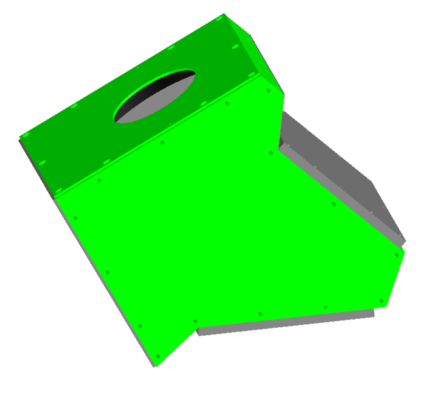
\includegraphics[width=0.6\linewidth]{Figures/cad1.pdf}
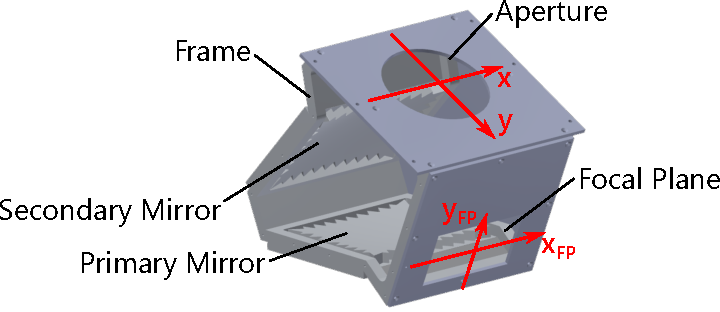
\includegraphics[width=0.8\linewidth]{Figures/LFT_BBM_CAD.pdf}
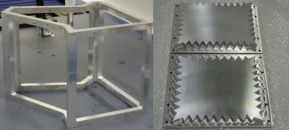
\includegraphics[width=0.9\linewidth]{Figures/Frame_and_Mirrors.pdf}
%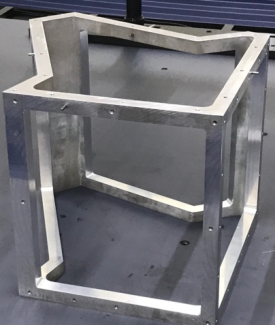
\includegraphics[width=0.6\linewidth]{Figures/frame.pdf}
%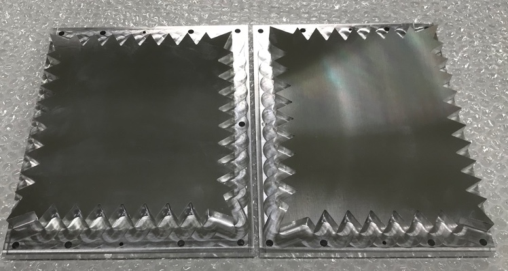
\includegraphics[width=0.6\linewidth]{Figures/mirrors.pdf}
\caption{(top) A cad model of the 1/4-scaled LFT. The optical design is symmetric in $x$ direction and asymmetric in $y$ direction. (bottom) The frame, primary mirror and secondary mirror. Serration is formed at the edges of the mirrors to reduce the diffraction.}
\label{fig:cad-frame-mirrors}
\end{figure}
\par
% \red{(Description of focal plane and wide field of view)}
The scaled LFT has a focal plane area of 100~mm $\times$ 50~mm to cover its wide FoV of $20^\circ \times 10^\circ$.  
Antenna patterns are measured at three positions of the focal plane as shown in Figure~\ref{fig:FeedPos}. For each position, the measurement was conducted for two orthogonal polarization directions, H-pol (horizontal polarization) and V-pol (vertical polarization).
%
\begin{figure}[!t]
\centering
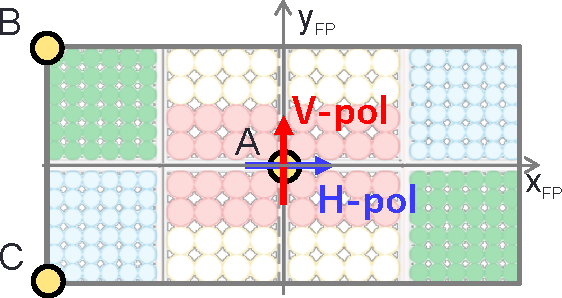
\includegraphics[width=0.8\linewidth]{Figures/FeedPos.pdf}
\caption{A schematic of the focal plane and feed positions. The colored circles show the positions and sizes of the lenslets. A, B and C show the positions where the feed is placed during the measurement, which are ($x_\mathrm{FP}$ /mm, $y_\mathrm{FP}$ /mm) = (0, 0), (-48.75, 23.25), (-48.75, 23.25) on the focal plane. H-pol and V-pol are two orthogonal polarization directions of the feed horn.}
\label{fig:FeedPos}
\end{figure}
%
%During the measurement, the conical horn antenna was placed at three positions on the focal plane, as shown in Figure~\ref{fig:FeedPos}. For each feed horn position, the measurement was conducted for two orthogonal polarization directions, V-pol (vertical polarization) and H-pol (horizontal polarization).
%
\subsection{Mechanical Errors}
%
We have studied the manufacturing tolerance using Synopsys Code~V. 
%\sout{This study \red{(reported at Annual Meeting of Astronomical Society of Japan 2019 Spring by Kashima-san)} shows that the manufacturing tolerance is limited by rotation tolerance of the polarization direction.}
Based on this study, we have defined the manufacturing tolerance as 1~mm and 30~arcsec for the translational and rotational errors respectively, for both the primary and secondary mirrors (see Table \ref{tb:mech_err}).
\par
To check whether the scaled LFT satisfies these requirement, the alignment accuracy and surface accuracy of the mirrors were measured by a 3-dimensional coordinate measuring machine (Mitsutoyo LEGEX 12128) with a contact probe. 100 points on the surface of each mirror were measured. 
As shown in Table \ref{tb:mech_err}, the translational and rotational errors were \red{$XX~\mathrm{\mu m}$} and \red{XX~arcsec} at the maximum respectively. The surface accuracy was \red{$XX~\mathrm{\mu m}$} rms for the primary mirror and \red{$XX~\mathrm{\mu m}$} rms for the secondary mirror. These numbers satisfy the defined tolerance. The surface roughness was also low enough to reduce the error patterns that create far-sidelobes.

%
\begin{table}[!t]
% increase table row spacing, adjust to taste
\renewcommand{\arraystretch}{1.3}
% if using array.sty, it might be a good idea to tweak the value of
% \extrarowheight as needed to properly center the text within the cells
\caption{Mechanical Errors of the Scaled Model}
\label{tb:mech_err}
\centering
% Some packages, such as MDW tools, offer better commands for making tables
% than the plain LaTeX2e tabular which is used here.
\begin{tabular}{|c|ccc|ccc|}
\hline
Mirror & \multicolumn{3}{|c}{Translational Error /mm} & \multicolumn{3}{|c|}{Rotational Error /arcsec} \\
 & $x$ & $y$ & $z$ & $\phi_x$ & $\phi_y$ & $\phi_z$ \\
\hline
Primary & XX & YY & ZZ & XX & YY & ZZ \\
(Tolerance) & XX & YY & ZZ & XX & YY & ZZ \\
\hline
Secondary & XX & YY & ZZ & XX & YY & ZZ \\
(Tolerance) & XX & YY & ZZ & XX & YY & ZZ \\
\hline
\end{tabular}
\end{table}
%
% (End of 1/4-scaled model)
%
\section{Measurement system}
%
\subsection{Near-field Beam Measurement System}
\par
A near-field beam measurement system based on a vector network analyzer (VNA) has been developed to characterize the scaled LFT (Figure~\ref{fig:MeasSys}). 
The VNA consists of a microwave part (Keysight N5222B) and WR5.1 frequency extenders (140--220~GHz) of transmitter and receiver modules (Virginia Diodes Inc.).
Since the LFT has been scaled in 1/4 dimension, the measurement wavelength must be accordingly scaled. We have therefore chosen the measurement frequencies as 140, 160, 180, 200 and 220~GHz, which correspond to 35--55~GHz of the full-scale LFT. 
This frequency range roughly corresponds to the lowest frequencies of LFT bands,
%named LF1 (34--99~GHz) with a lens diameter of 24 mm and \red{MF1 (60--137~GHz)} with a lens diameter of 16 mm, 
at which larger far-sidelobes are expected due to diffraction.  
%
\par
A probe horn with the receiver module measures both the amplitude and phase distributions near the aperture with an $XY\Phi$ scanner. The maximum travel length of the scanner is 300~mm with the flatness of $<25~\mathrm{\mu m}$ for each axis. As the probe horn, a \red{WR6} open-ended waveguide has been used. Its aperture is 1.651~mm $\times$ 0.8255~mm rectangular shape with tapered edges to reduce the return loss. The polarization direction of the probe horn can be rotated.
A horn with the transmitter module is placed at an arbitrary position on the focal plane with an $XYZ$ stage, whose travel length is 200~mm $\times$ 75~mm $\times$ 30~mm.
A dedicated Python script has been developed to control the system using PyVISA package\footnote{https://pyvisa.readthedocs.io/}.
Note that this arrangement is a time-reversed configuration of a real CMB observation.
%
\begin{figure}[!t]
\centering
\includegraphics[width=0.9\linewidth]{Figures/MeasSys.pdf}
\caption{The 1/4-scaled model of LFT and its near-field beam measurement system. A conical horn with the transmitter of a vector network analyzer scans the focal plane of the scaled LFT with the XYZ stage. A probe horn with the receiver measures the amplitude and phase distributions near the aperture with the XY$\Phi$ stage. 
% The system is controlled by a dedicated Python script.
}
\label{fig:MeasSys}
\end{figure}
%
%
\subsection{Feed Horn}
\par
The focal plane of LiteBIRD LFT has TES bolometer arrays with sinuous antennas and lenslets, whose diameter is 24~mm for the 34--87~GHz bands and 16~mm for the \red{60}--161~GHz bands~\cite{Suzuki2018}. 
Their beam patterns have been characterized in that a main lobe has a shape of a Gaussian beam~\cite{Edwards2012}. 
The optical design of LFT assumes Gaussian beams with the beam waist radius of 9.412~mm for the 34--87~GHz bands and 8.727~mm for the 60--161~GHz bands.
\par 
As a feed of the 1/4-scaled LFT, a smoothed-wall conical horn has been used instead, whose aperture diameter and length are 10.4~mm and 20~mm respectively. Its beam pattern has been measured in advance using a near-field beam scanner. The results are shown in Figure~\ref{fig:Feedhorn}. The measured beam width of the conical horn was $\lesssim 10\%$ larger at 180~GHz and $\lesssim 15\%$ larger at 140 and 220~GHz than that of the Gaussian-approximated beam patterns of the actual focal plane arrays.

\begin{figure}[!t]
\centering
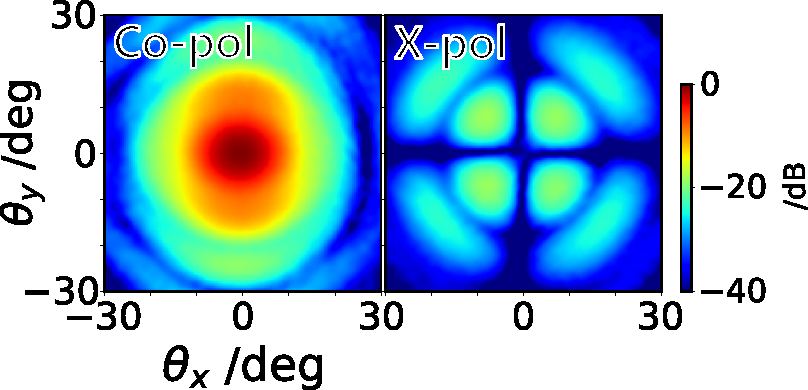
\includegraphics[width=0.9\linewidth]{Figures/FeedHornPattern.pdf}
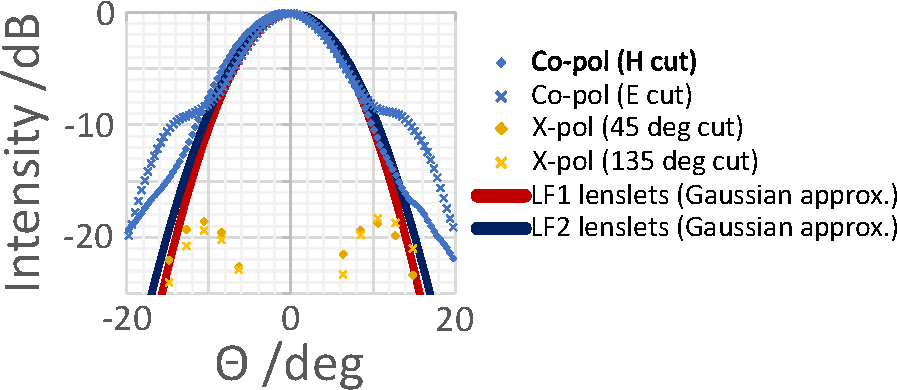
\includegraphics[width=0.9\linewidth]{Figures/FeedHorn_vs_Lenslet.pdf}
\caption{%
(top) The measured beam patterns of a conical horn used as the feed at 180~GHz (corresponding to 45~GHz of the full-scale model). Co-pol and X-pol stand for co-polarization and cross-polarization respectively. The E-plane is parallel to the $\theta_y$ axis. The maximum cross-polarization level is -17~dB.
(bottom) The dots show the $\theta_y = 0$ cut ($\phi = 0$; H cut) and $\theta_x = 0$ cut ($\phi = 90^\circ$; E cut) of the measured co-polarization beam patterns of the conical horn at 180~GHz, as well as $\phi=45^\circ$ and $\phi=135^\circ$ cuts of the measured cross-polarization patterns. The solid lines show the Gaussian beams, which are an approximation to the beam patterns of the actual focal plane arrays with sinuous antennas and lenslets.
}
\label{fig:Feedhorn}
\end{figure}
%
% (End of Measurement System)
%
\section{Data Processing}
%
%\subsection{Coordinates}%This subsection was merged to Fig. 1.]}
%\par
%We have adopted right-handed coordinates system defined as follows: $z$ axis corresponds to the optical axis of LFT, whose direction is from the aperture to the focal plane. $x_\mathrm{FP}$ and $y_\mathrm{FP}$ are defined on the focal plane as shown in Figure~\ref{fig:FeedPos}. $x$ and $y$ are defined on the aperture plane such that $x$ axis is parallel to $x_\mathrm{FP}$ axis. $\theta_x$ and $\theta_y$ are the angle from $z$ axis toward $x$ and $y$ axes, and $\phi$ is the angle in the $xy$ plane measured from $x$ axis.
%\par
%Coordinates for cross-polarization follow Ludwig's Definition 3 \cite{Ludwig1973}.
%
%\subsection{Linearity Calibration}
The linearity of the VNA has been corrected with an attenuator (Elmika DA-015E) which had been calibrated down to -50~dB. 
%We have evaluated the measurement errors at 12 different levels down to -70~dB. 
Combined with a fixed waveguide attenuator, the measured near-field amplitudes have been calibrated with a dynamic range of 75~dB.
%
%\subsection{Time Variation Compensation}
In addition, to reduce the effects of time variation of VNA, the amplitude and phase at a reference position are monitored every 15~minutes during the measurement. The amplitude and phase variations have been compensated with the accuracy of $\lesssim \pm 0.1 \ \mathrm{dB}$ and $\lesssim \pm 4^\circ$.
%
%\subsection{Near- to Far-field Transformation}
\par
The far-field beam pattern is a complex Fourier transformation of the measured near-field amplitude and phase maps. Fast Fourier Transform (FFT) algorithm~\cite{Cooley1965} is used to calculate this near- to far-field transformation. The measured near-field maps with 360 $\times$ 360 points are zero-padded to 512 $\times$ 512 points before applying FFT.
%
%\subsection{Probe Correction}
%
%An open-ended waveguide was used as the probe horn.
The far-field patterns have been corrected with the far-field patterns of the probe horn, which are calculated analytically following the formulas in \cite{Yaghjian1984}. 
%
% (End of Data Processing)
%
\section{Results and Discussion}
%
\subsection{Near-field Measurements}
%
A set of the measured amplitude and phase maps is shown in Figure~\ref{fig:NF_f1_Vpol}. They are probed every 0.5~mm in a rectangular area of $180 \times 180~\mathrm{mm}$, 15~mm beneath the bottom of the hood. The probe horn was moved from $-x$ to $+x$ direction for each $y$ coordinate. The sampling spacing was determined so as to satisfy the Nyquist condition. %\red{The measurement area is optimized in advance to get a far-field beam pattern with errors of less than -70~dB level. ?} 
A scan takes around 30 hours to obtain a set of 5-frequency near-field patterns for each feed horn position and one polarization angle, which may be reduced by optimizing the sequence of the data acquisition.
%
\par
The area whose amplitude is more than -40~dB has been fully sampled. In the phase maps, small variations up to $\sim 4^\circ$ were observed even after the time variation calibration. This is because the timescale of the phase variation is shorter than the interval of measuring the reference position ($\sim 15$ minutes). 
The variation was larger in $y$ direction, which is orthogonal to the scanning direction.
\begin{figure}[!t]
\centering
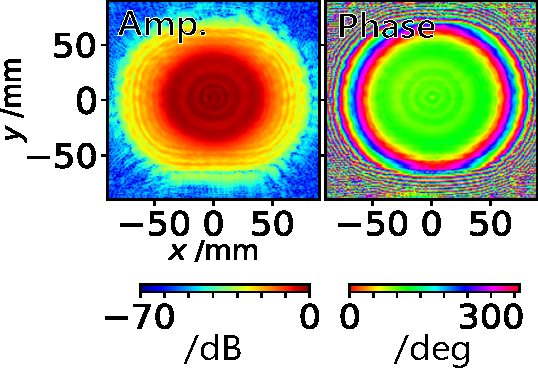
\includegraphics[width=\linewidth]{Figures/NF_f1_Vpol.pdf}
\hfil
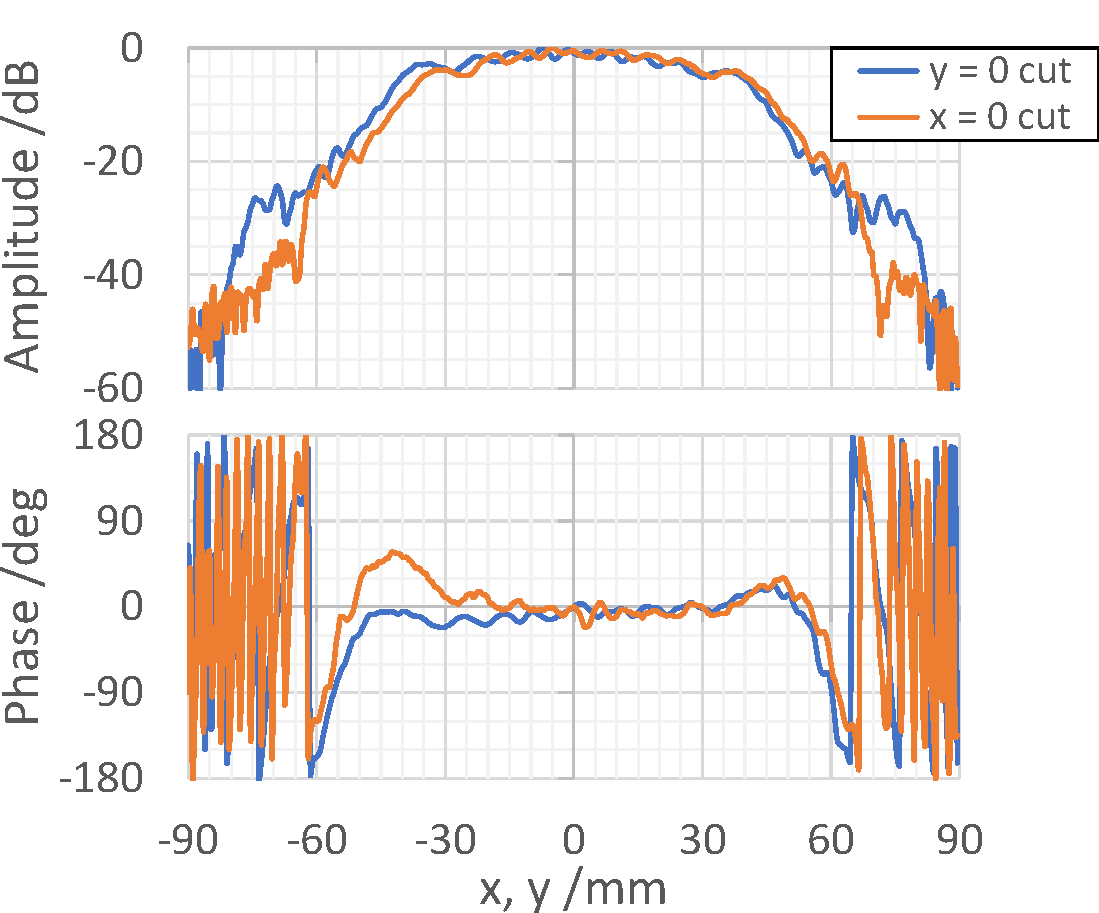
\includegraphics[width=0.8\linewidth]{Figures/NF_f1_Vpol_cut.pdf}
\caption{%
(top) Amplitude and phase maps measured 15~mm beneath the aperture. 140, 160, 180, 200 and 220~GHz are measured simultaneously. The feed horn is placed at Position A.
(bottom) $\theta_y = 0$ and $\theta_x = 0$ cuts of amplitude and phase maps at 180~GHz. Note that the phase is shifted. 
}
\label{fig:NF_f1_Vpol}
\end{figure}
%
%%%
%
\subsection{Comparison with Simulation}
%
%\red{Pls move this paragraph to a section of LFT scaled model. \\
%Former studies \cite{Kashima2018, Imada2018} had predicted that some far-sidelobe components would be created due to stray light, such as direct rays from the sky to the focal plane and three-time reflected rays. These sidelobes are designed to be reduced by the hood attached on the aperture (see Figure~\ref{fig:MeasSys}).}
\par
Figure~\ref{fig:Hood_F1_140G} shows the beam patterns at 140~GHz measured without and with the hood, and their $\theta_y = 0$ and $\theta_x = 0$ cuts. Note that $\theta_x$ and $\theta_y$ are the angles from the optical axis toward $x$ and $y$ axes. For without-hood case, sidelobe components caused by stray light are observed at $\theta_y \sim -50^\circ$ and $\theta_y \sim 40^\circ$, which correspond to direct rays and three-time reflected rays, respectively. These far-sidelobe features are reduced by around 20~dB when measured with the hood.
\par
Figure~\ref{fig:Hood_F1_140G} also shows the calculated beam pattern of the scaled LFT at 140~GHz without including the effects of the stray light. The calculation is based on \cite[Eq. 1.22]{Kitsuregawa1990}. The measured beam pattern with the hood agrees with the calculated beam pattern without stray light at down to -50~dB level. 
%
\begin{figure}[!t]
\centering
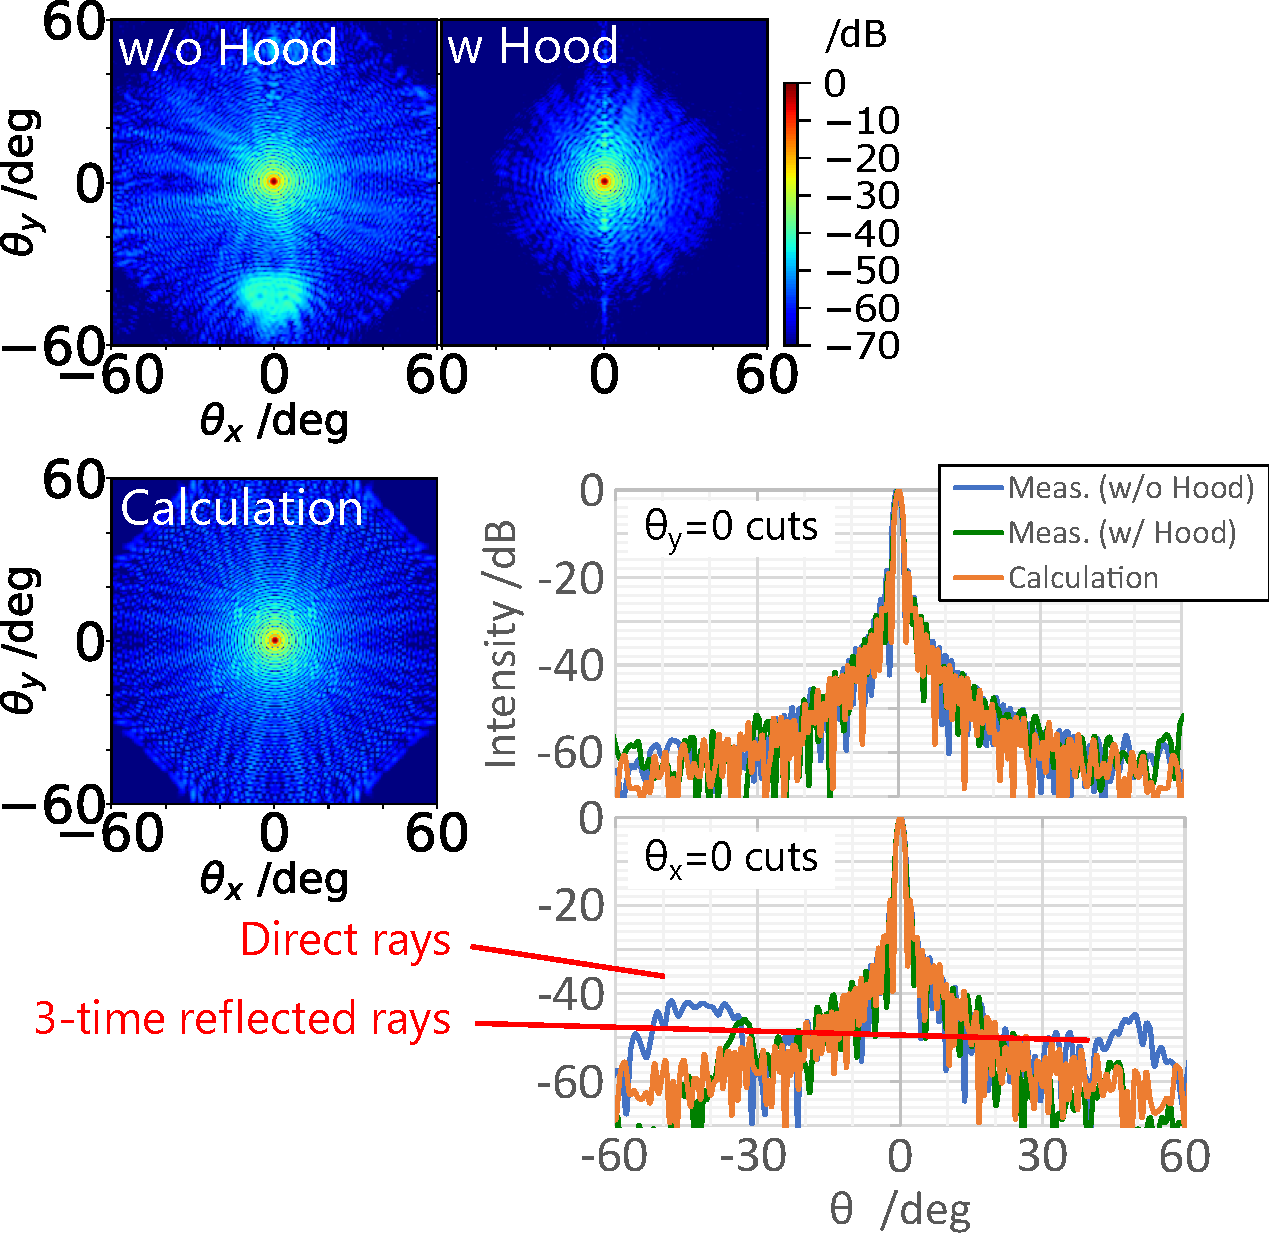
\includegraphics[width=\linewidth]{Figures/Hood_F1_140G.pdf}
%\hfil
%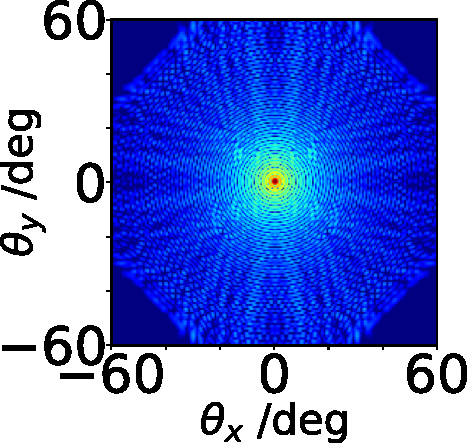
\includegraphics[width=0.45\linewidth]{Figures/Calc_F1_140G.pdf}
%\hfil
%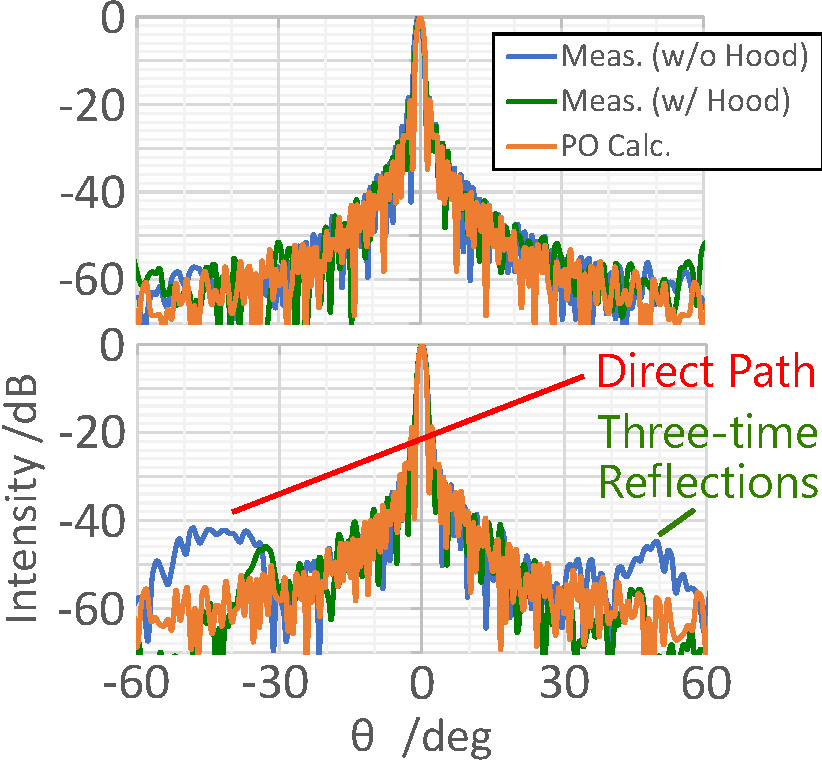
\includegraphics[width=0.5\linewidth]{Figures/Hood_F1_140G_cut.pdf}
\caption{%
(top) The beam patterns at 140~GHz (corresponds to 35~GHz) measured without and with the hood. The feed horn was placed at Position A. \red{To be replaced with 180~GHz results, for comparison with X-pol maps.}
(bottom) A calculated beam pattern for Position~A at 140~GHz. The calculation is for without-hood case and does not include the effects of stray light.
Their $\theta_y = 0$ cuts and $\theta_x = 0$ cuts are compared with the measurement results. 
%\protect\linebreak
For without-hood case, sidelobe components caused by stray light are observed at $\theta_y \sim -50^\circ$ and $\theta_y \sim 40^\circ$, which correspond to direct rays from the sky to the focal plane and three-time reflected rays respectively. For with-hood case, these far-sidelobe features are drastically reduced; the measured beam pattern shows good agreement with the calculated beam pattern without stray light.
}
\label{fig:Hood_F1_140G}
\end{figure}
%
%%%
\subsection{Far-sidelobe Patterns}
%
Measured far-field beam patterns at the feed horn positions of A, B and C are shown in Figure~\ref{fig:HVpol_140G} (140~GHz) and Figure~\ref{fig:HVpol_220G} (220~GHz). 
Frequency dependence of far-sidelobes from 140~GHz to 220~GHz (corresponding to 35--55~GHz) has been confirmed to be small.
The vertical features at $\theta_x \sim 0^\circ$ with a level of $\sim -50~\mathrm{dB}$ have been identified as near-field scanning noise caused by remaining time variation of the phase during the measurement. 
\par
The measurements have confirmed that the far-sidelobe components outside of $\sim \pm25^\circ$ are mostly suppressed down to -56~dB level, except for some small-scale features caused by the remaining stray light. Also, beam patterns of two orthogonal polarization directions, H-pol and V-pol, are found to be consistent with each other at down to -40 dB level even at the edges of the focal plane, namely feed horn positions of B and C.
%
\begin{figure}[!t]
\centering
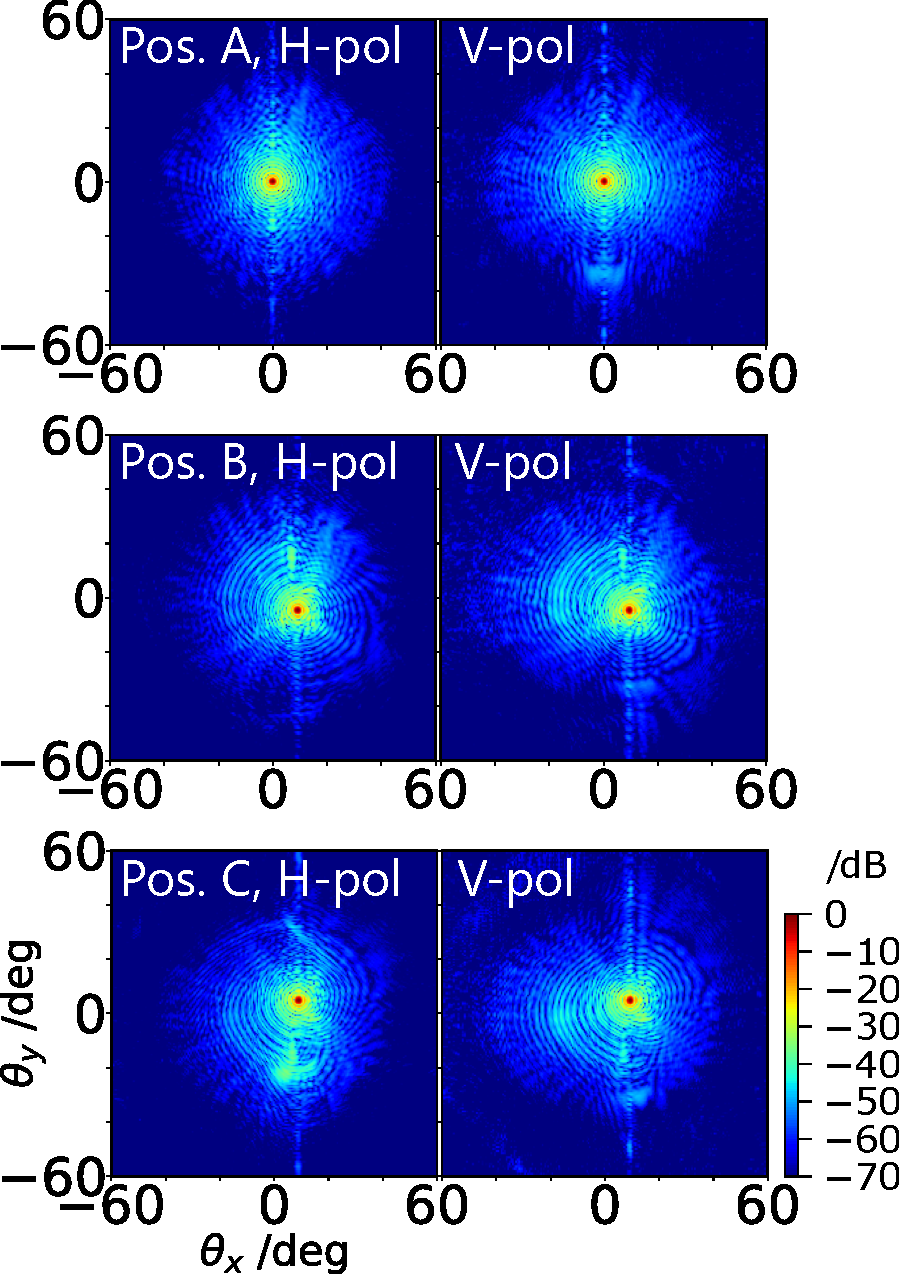
\includegraphics[width=0.9\linewidth]{Figures/HVpol_140G.pdf}
\hfil
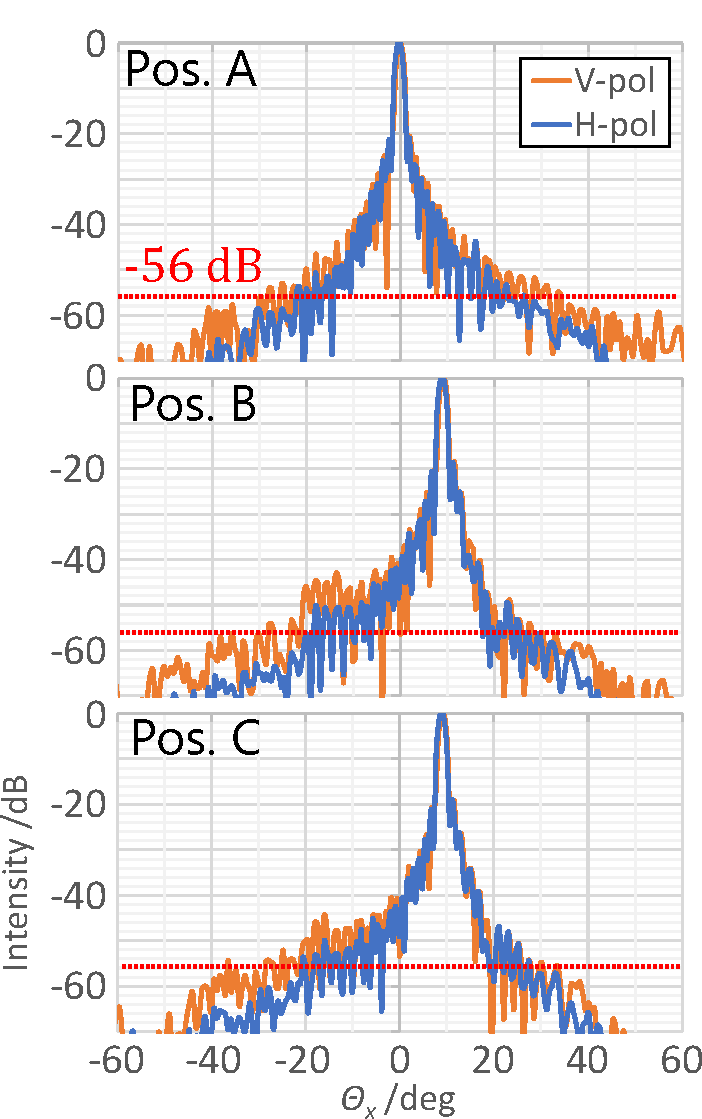
\includegraphics[width=0.7\linewidth]{Figures/HVpol_140G_Xcut}
\caption{%
(top) H-pol and V-pol beam patterns at each feed horn position of A, B and C, measured at 140~GHz. 
(bottom) Their $theta_y = 0$, \red{$\theta_y = -4.8^\circ$ and $\theta_y = 4.3^\circ$} cuts.
}
\label{fig:HVpol_140G}
\end{figure}
%
\begin{figure}[!t]
\centering
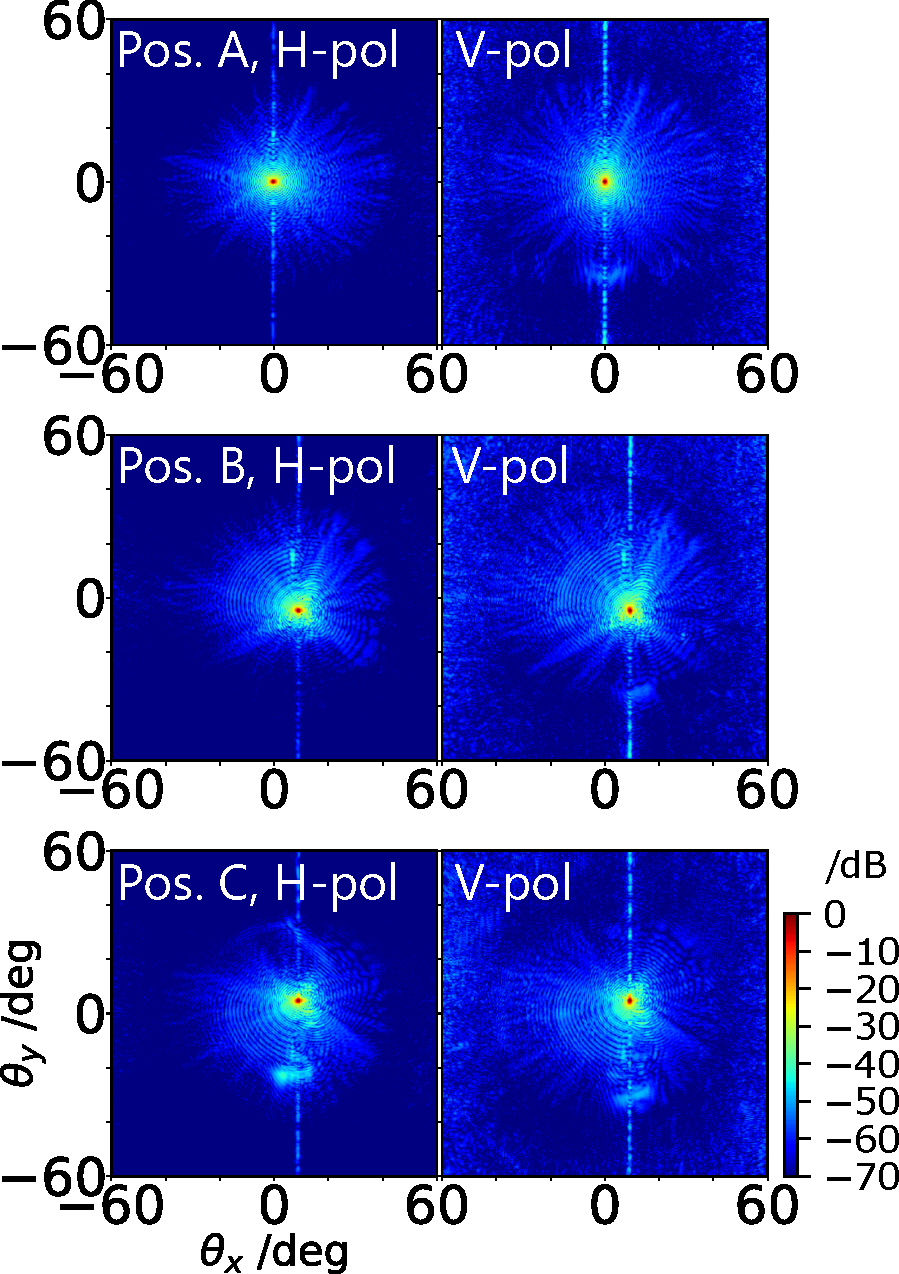
\includegraphics[width=0.9\linewidth]{Figures/HVpol_220G.pdf}
\hfil
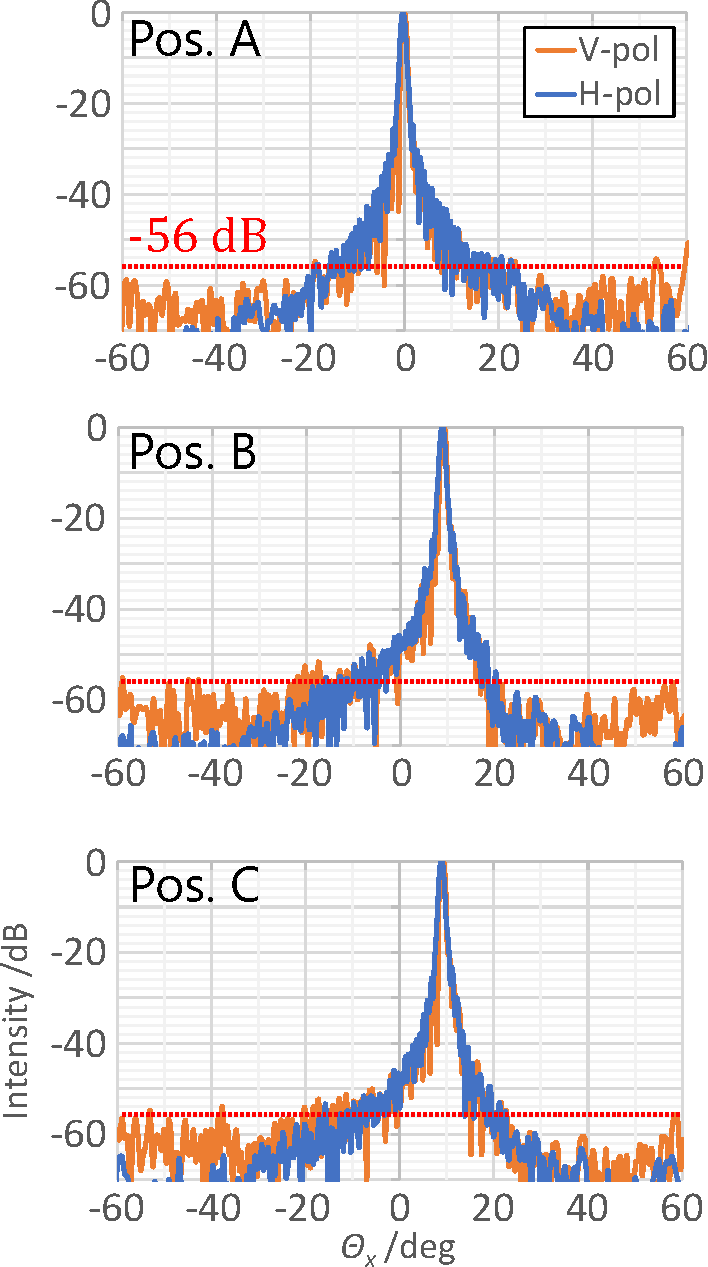
\includegraphics[width=0.7\linewidth]{Figures/HVpol_220G_Xcut}
\caption{%
(top) H-pol and V-pol beam patterns at each feed horn position of A, B and C, measured at 220~GHz. 
(bottom) Their $\theta_y = 0$, $\theta_y = -4.6^\circ$ and $\theta_y = 4.6^\circ$ cuts.
}
\label{fig:HVpol_220G}
\end{figure}
%
%%%
\subsection{Cross-polarization patterns}
%
Measured cross-polarization patterns for feed horn positions of A, B and C at 180~GHz are shown in Figure~\ref{fig:HVpol_Xpol_180G}.
Note that the coordinates for cross-polarization follow Ludwig's Definition 3 \cite{Ludwig1973}.
Frequency dependence of the cross-polarization patterns from 140~GHz to 220~GHz (corresponding to 35--55~GHz) has been confirmed to be small.
The peak level of cross-polarization is less than -20 dB regardless of the feed horn position nor the polarization direction. The patterns show four peaks in diagonal directions, which are consistent with those of the conical horn used as the feed (see Figure~\ref{fig:Feedhorn}).
\par
%To evaluate the cross-polarization caused by the LFT mirrors themselves, we have also measured cross-polarization patterns with placing a free standing wire grid polarizer (Microtech Instruments G30x10-S) between the feed horn and the LFT scaled model. 
To evaluate cross polarization caused by the conical horn, a free-standing wire-grid (Microtech instruments G30x10-S) has been placed in front of the conical horn, which reduces the cross polarization of the conical horn.
The results are shown in Figure~\ref{fig:HVpol_Xpol_180G_wiregrid}. 
From these results, we have confirmed that the cross-polarization of the scaled LFT (Figure \ref{fig:HVpol_Xpol_180G}) is caused mostly from the conical horn.
The cross-polarization created by the scaled LFT itself is verified to be less than -35~dB.
Intensity ratio of cross-polarization and co-polarization in the far-sidelobes has been demonstrated to be less than -10 dB. It is preferable for CMB polarization observations.
%
\begin{figure}[!t]
\centering
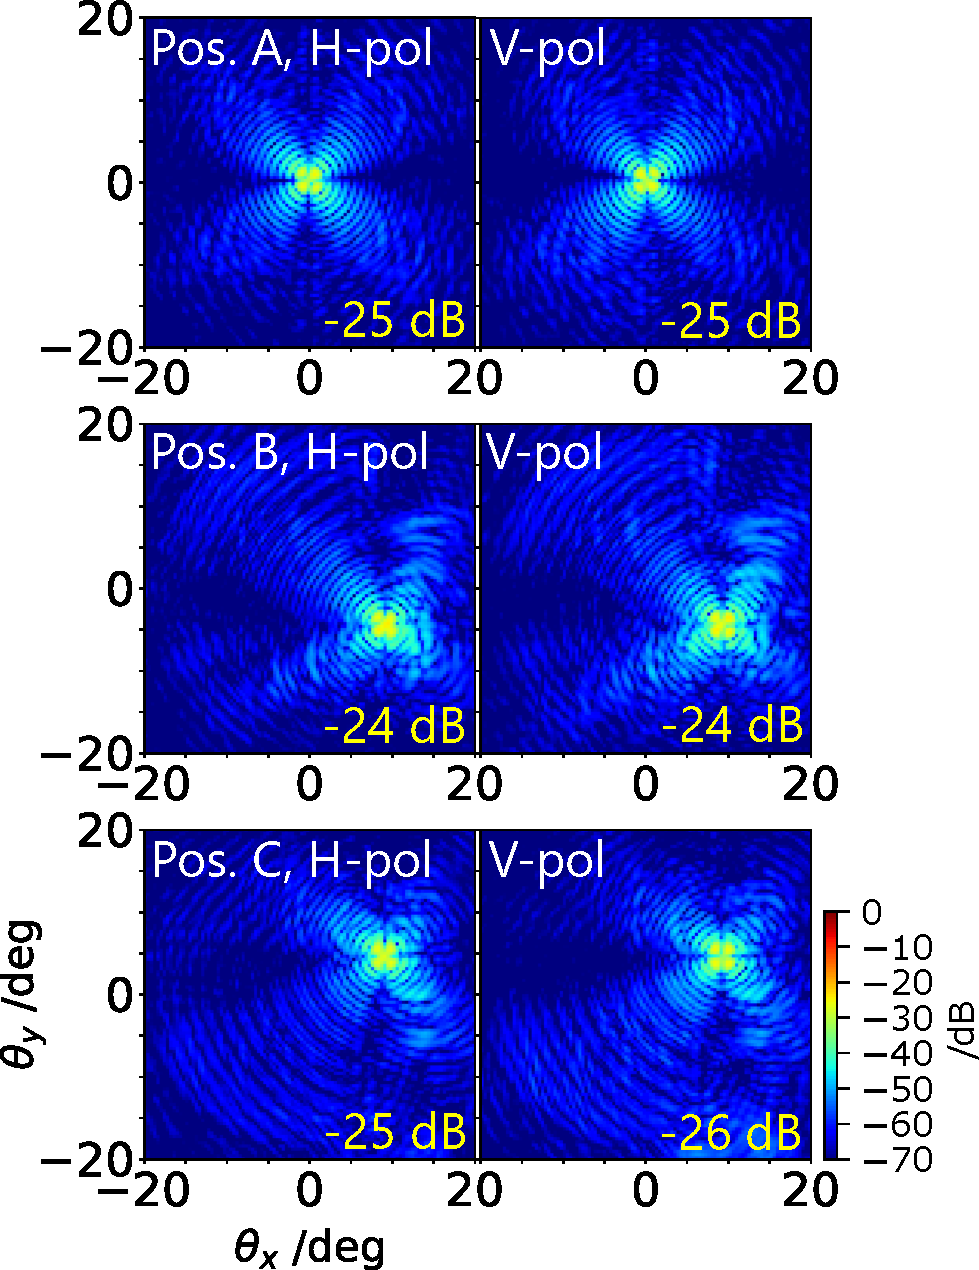
\includegraphics[width=\linewidth]{Figures/HVpol_Xpol_180G.pdf}
\caption{%
Cross-polarization beam patterns for H-pol and V-pol at each feed horn position of A, B and C, measured at 180~GHz. The values show the peak level of the cross-polarization.
}
\label{fig:HVpol_Xpol_180G}
\end{figure}
%
\begin{figure}[!t]
\centering
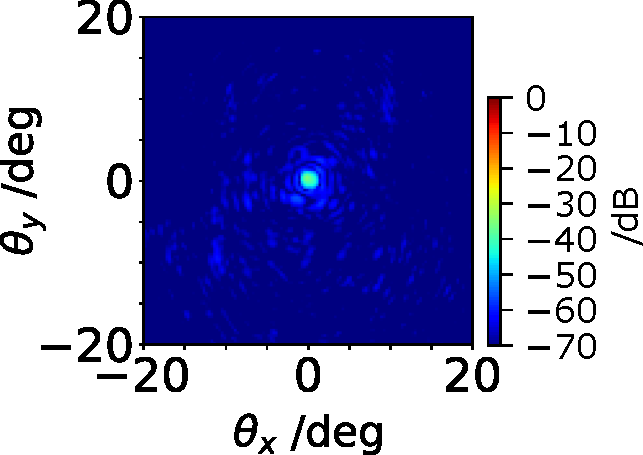
\includegraphics[width=0.7\linewidth]{Figures/HVpol_Xpol_180G_wiregrid.pdf}
\hfil
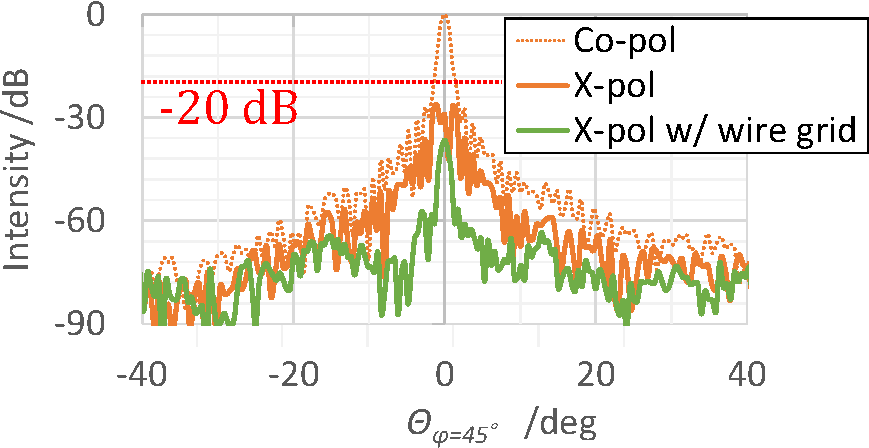
\includegraphics[width=0.9\linewidth]{Figures/HVpol_Xpol_180G_cut.pdf}
\caption{%
(top) Cross-polarization beam pattern for V-pol at Position A, measured with a wire grid polarizer at 180~GHz. The peak level was -35~dB.
(bottom) $\theta_y = 0$ cut of V-pol co-polarization pattern, and $\phi = 45^\circ$ cuts of V-pol cross-polarization patterns without and with wire grid polarizer.
}
\label{fig:HVpol_Xpol_180G_wiregrid}
\end{figure}
%
% (End of Results and Discussion)
%
\section{Summary}
We have developed a 1/4-scaled model of LiteBIRD LFT and its near-field beam measurement system to confirm the far-sidelobe patterns of LFT. We have measured beam patterns for two orthogonal polarization directions at the center and the edges of the focal plane. The measurement frequency was 140-220 GHz, which correspond to the lowest bands (35-55 GHz) of the full-scale LFT.
\par
The measurements are consistent with the simulated far-sidelobe patterns at -50~dB level, and have confirmed that some far-sidelobe features are due to stray light and are drastically reduced by the hood. Other far-sidelobe components are mostly less than -56 dB. We have also found that beams for two orthogonal polarization directions are consistent with each other down to -40~dB level. The cross-polarization level has also been measured to be less than -20 dB, most of which is originated from the cross-polarization of the feed horn.
%
% (End of Summary)
%
%
% An example of a floating figure using the graphicx package.
% Note that \label must occur AFTER (or within) \caption.
% For figures, \caption should occur after the \includegraphics.
% Note that IEEEtran v1.7 and later has special internal code that
% is designed to preserve the operation of \label within \caption
% even when the captionsoff option is in effect. However, because
% of issues like this, it may be the safest practice to put all your
% \label just after \caption rather than within \caption{}.
%
% Reminder: the "draftcls" or "draftclsnofoot", not "draft", class
% option should be used if it is desired that the figures are to be
% displayed while in draft mode.
%
%\begin{figure}[!t]
%\centering
%\includegraphics[width=2.5in]{myfigure}
% where an .eps filename suffix will be assumed under latex, 
% and a .pdf suffix will be assumed for pdflatex; or what has been declared
% via \DeclareGraphicsExtensions.
%\caption{Simulation results for the network.}
%\label{fig_sim}
%\end{figure}
%
% Note that the IEEE typically puts floats only at the top, even when this
% results in a large percentage of a column being occupied by floats.
%
% An example of a double column floating figure using two subfigures.
% (The subfig.sty package must be loaded for this to work.)
% The subfigure \label commands are set within each subfloat command,
% and the \label for the overall figure must come after \caption.
% \hfil is used as a separator to get equal spacing.
% Watch out that the combined width of all the subfigures on a 
% line do not exceed the text width or a line break will occur.
%
%\begin{figure*}[!t]
%\centering
%\subfloat[Case I]{\includegraphics[width=2.5in]{box}%
%\label{fig_first_case}}
%\hfil
%\subfloat[Case II]{\includegraphics[width=2.5in]{box}%
%\label{fig_second_case}}
%\caption{Simulation results for the network.}
%\label{fig_sim}
%\end{figure*}
%
% Note that often IEEE papers with subfigures do not employ subfigure
% captions (using the optional argument to \subfloat[]), but instead will
% reference/describe all of them (a), (b), etc., within the main caption.
% Be aware that for subfig.sty to generate the (a), (b), etc., subfigure
% labels, the optional argument to \subfloat must be present. If a
% subcaption is not desired, just leave its contents blank,
% e.g., \subfloat[].
%
% An example of a floating table. Note that, for IEEE style tables, the
% \caption command should come BEFORE the table and, given that table
% captions serve much like titles, are usually capitalized except for words
% such as a, an, and, as, at, but, by, for, in, nor, of, on, or, the, to
% and up, which are usually not capitalized unless they are the first or
% last word of the caption. Table text will default to \footnotesize as
% the IEEE normally uses this smaller font for tables.
% The \label must come after \caption as always.
%
%\begin{table}[!t]
%% increase table row spacing, adjust to taste
%\renewcommand{\arraystretch}{1.3}
% if using array.sty, it might be a good idea to tweak the value of
% \extrarowheight as needed to properly center the text within the cells
%\caption{An Example of a Table}
%\label{table_example}
%\centering
%% Some packages, such as MDW tools, offer better commands for making tables
%% than the plain LaTeX2e tabular which is used here.
%\begin{tabular}{|c||c|}
%\hline
%One & Two\\
%\hline
%Three & Four\\
%\hline
%\end{tabular}
%\end{table}
%
% Note that the IEEE does not put floats in the very first column
% - or typically anywhere on the first page for that matter. Also,
% in-text middle ("here") positioning is typically not used, but it
% is allowed and encouraged for Computer Society conferences (but
% not Computer Society journals). Most IEEE journals/conferences use
% top floats exclusively. 
% Note that, LaTeX2e, unlike IEEE journals/conferences, places
% footnotes above bottom floats. This can be corrected via the
% \fnbelowfloat command of the stfloats package.
%

%
% if have a single appendix:
%\appendix[Proof of the Zonklar Equations]
% or
%\appendix  % for no appendix heading
% do not use \section anymore after \appendix, only \section*
% is possibly needed
%
% use appendices with more than one appendix
% then use \section to start each appendix
% you must declare a \section before using any
% \subsection or using \label (\appendices by itself
% starts a section numbered zero.)
%
%
% \appendices
% \section{Proof of the First Zonklar Equation}
% Appendix one text goes here.
%
% you can choose not to have a title for an appendix
% if you want by leaving the argument blank
% \section{}
% Appendix two text goes here.
%
%
% use section* for acknowledgment
\section*{Acknowledgment}
%
The authors would like to acknowledge Tetsuya Ito, Yoshinori Uzawa (NAOJ) and Tom Nitta (Univ. of Tsukuba) for 
their kind advice on design of near-field beam measurement system. We also would like to thank LiteBIRD Pre-phase A2 members for their many pieces of advice and discussion.
\par
This work was supported by 
the acceleration program of JAXA research and development directorate,
NAOJ support program, and
JSPS/MEXT KAKENHI Grant Numbers JP17H01115, JP15H05891, JP15H05743.
%The measurement is supported by an acceleration program of JAXA research and development directorate.
%
% Can use something like this to put references on a page
% by themselves when using endfloat and the captionsoff option.
\ifCLASSOPTIONcaptionsoff
  \newpage
\fi
%
% trigger a \newpage just before the given reference
% number - used to balance the columns on the last page
% adjust value as needed - may need to be readjusted if
% the document is modified later
%\IEEEtriggeratref{8}
% The "triggered" command can be changed if desired:
%\IEEEtriggercmd{\enlargethispage{-5in}}
%
% references section
%
% can use a bibliography generated by BibTeX as a .bbl file
% BibTeX documentation can be easily obtained at:
% http://mirror.ctan.org/biblio/bibtex/contrib/doc/
% The IEEEtran BibTeX style support page is at:
% http://www.michaelshell.org/tex/ieeetran/bibtex/
\bibliographystyle{IEEEtran}
% argument is your BibTeX string definitions and bibliography database(s)
%
% "Each reference cited must have a complete list of authors (no et al.), complete titles, first and last pages numbers, month and year. In addition, authors are required to include the Digital Object Identifier (DOI)." (https://www.mtt.org/terahertz/)
\bibliography{ISSTT_Proceedings.bib}
%
%
% biography section
% 
% If you have an EPS/PDF photo (graphicx package needed) extra braces are
% needed around the contents of the optional argument to biography to prevent
% the LaTeX parser from getting confused when it sees the complicated
% \includegraphics command within an optional argument. (You could create
% your own custom macro containing the \includegraphics command to make things
% simpler here.)
%\begin{IEEEbiography}[{\includegraphics[width=1in,height=1.25in,clip,keepaspectratio]{mshell}}]{Michael Shell}
% or if you just want to reserve a space for a photo:
%
\begin{IEEEbiography}{Hayato Takakura}
received the B.S. degree in physics from Keio University, Yokohama, Japan in 2014. Since then, he has been with Institute of Space and Astronautical Science (ISAS), Japan Aerospace Exploration Agency (JAXA), Sagamihara, Japan, as a graduate student in the Department of Astronomy, School of Science, the University of Tokyo. His research interests include the area of millimeter-wave optics.
\end{IEEEbiography}
%
% if you will not have a photo at all:
%
\begin{IEEEbiographynophoto}{Yutaro Sekimoto}
received the Ph.D. degree from School of Science, University of Tokyo, Japan in 1994. 
He has been with ISAS/JAXA since 2017.
His research interests cover CMB B-mode polarization observations and millimeter-wave instrumentation.
\end{IEEEbiographynophoto}
%
\begin{IEEEbiographynophoto}{Junji Inatani}
Biography text here.
\end{IEEEbiographynophoto}
%
\begin{IEEEbiographynophoto}{Shingo Kashima}
Biography text here.
\end{IEEEbiographynophoto}
%
\begin{IEEEbiographynophoto}{Hiroaki Imada}
Biography text here.
\end{IEEEbiographynophoto}
%
\begin{IEEEbiographynophoto}{Takashi Hasebe}
Biography text here.
\end{IEEEbiographynophoto}
%%
\begin{IEEEbiographynophoto}{Toru Kaga}
Biography text here.
\end{IEEEbiographynophoto}
%
\begin{IEEEbiographynophoto}{Yoichi Takeda}
Biography text here.
\end{IEEEbiographynophoto}
%
%
\begin{IEEEbiographynophoto}{Norio Okada}
Biography text here.
\end{IEEEbiographynophoto}
% You can push biographies down or up by placing
% a \vfill before or after them. The appropriate
% use of \vfill depends on what kind of text is
% on the last page and whether or not the columns
% are being equalized.
%
%\vfill
%
% Can be used to pull up biographies so that the bottom of the last one
% is flush with the other column.
%\enlargethispage{-5in}
%
\end{document}